\documentclass{article}
\usepackage[utf8]{inputenc}
\usepackage{amsmath}
\usepackage{graphicx}
\usepackage{float}
\usepackage[font=scriptsize,labelfont=bf]{caption}

\title{COMP6245 : Lab 3 Report}
\author{Thanakorn Panyapiang(tp2n19@soton.ac.uk)}
\date{}

\begin{document}
\maketitle

\section{Class Boundaries and Posterior Probability}
\begin{center}
\begin{tabular}{ccc}
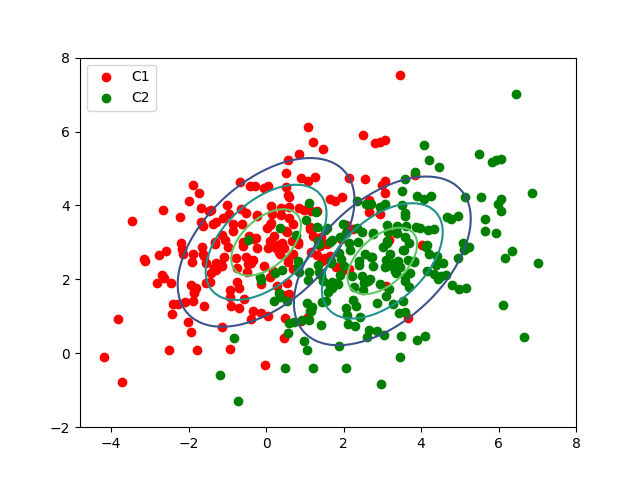
\includegraphics[scale=0.25]{y_scatter} &
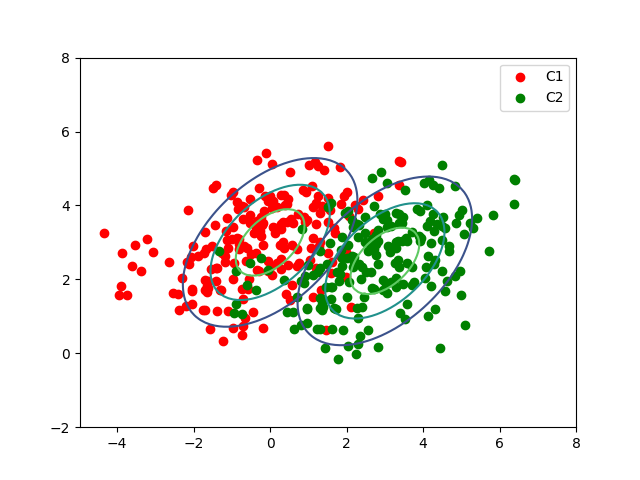
\includegraphics[scale=0.25]{z_scatter} &
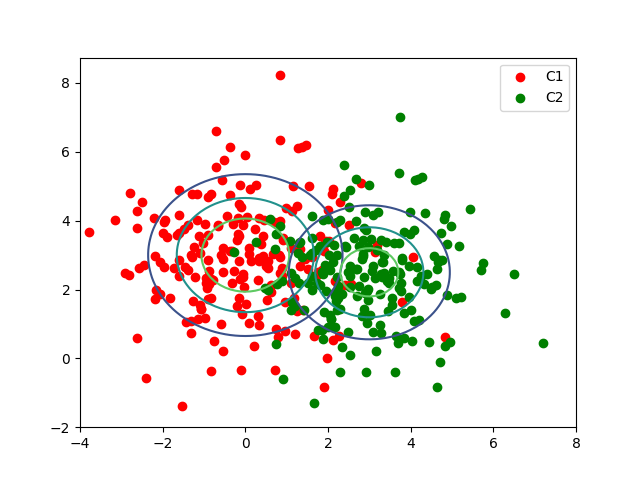
\includegraphics[scale=0.25]{w_scatter} \\
\scriptsize $\Sigma_{1} = \Sigma_{2} = \begin{bmatrix}2 & 1 \\ 1 & 2 \end{bmatrix}$ & 
\scriptsize $\Sigma_{1} = \Sigma_{2} = \begin{bmatrix}2 & 1 \\ 1 & 2 \end{bmatrix}$ &
\scriptsize $\Sigma_{1} = \begin{bmatrix}2 & 0 \\ 0 & 2 \end{bmatrix} \Sigma_{2} = \begin{bmatrix}1.5 & 0 \\ 0 & 1.5 \end{bmatrix}$\\
\scriptsize $P_{1} = P_{2} = 0.5$ & 
\scriptsize $P_{1} = 0.7, P_{2} = 0.3 $ &
\scriptsize $P_{1} = P_{2} = 0.5$\\
\end{tabular}
\captionof{figure}{}
\end{center}

Figure 1 illustrates the scatter of three classification problems which are drawn from different distributions.\\
\indent The class boundary is the area where the posterior probability of $\omega_{1}$ and $\omega_{2}$ are equal which can be written as an equation below:
\begin{equation} \label{eq:1}
P(\omega_{1} | x) = P (\omega_{2} | x)
\end{equation}

Since both classes have a Gaussian distribution, Eq. 1 can be define as:
\begin{equation} \label{eq:2}
P_{1}\frac{1}{{|\Sigma_{1}| 2\pi }}e^{{{ - \left({x - \mu_1} \right)^{T}\Sigma_1^{-1}({x - \mu_1}}) \mathord{\left/ {\vphantom {{ - \left( {x - \mu_{1} } \right)^2 } {2}}} \right. \kern-\nulldelimiterspace} {2}}} = P_{2}\frac{1}{{|\Sigma_{2}| 2\pi }}e^{{{ - \left({x - \mu_2} \right)^{T}\Sigma_2^{-1}({x - \mu_2}}) \mathord{\left/ {\vphantom {{ - \left( {x - \mu_2 } \right)^2 } {2}}} \right. \kern-\nulldelimiterspace} {2}}}
\end{equation}

As covariance matrix and the prior probabilities are equal on the first dataset. Eq. 2 can be simplified by eliminating all equal terms which results as follow.
$$
{{\left({x - \mu_1} \right)^{T}({x - \mu_1}})}  = {{\left({x - \mu_2} \right)^{T}({x - \mu_2}})}
$$
$$
{x^Tx - \mu_1^T\mu_1 - \mu_1^Tx - x^T\mu_1}  = {x^Tx - \mu_2^T\mu_2 - \mu_2^Tx - x^T\mu_2}
$$
\indent \textit{${x^T}$x} can be removed as it is on both sides, $\mu_1^T\mu_1$ and $\mu_2^T\mu_2$ are constant, and $\mu_1^Tx$  and $\mu_2^Tx$ are scalar, the decision boundary can be simplified to
$$x^T\mu_1 + C_1= x^T\mu_2 + C_2$$
\begin{equation} \label{eq:3}
x^T(\mu_1 - \mu_2) + C = 0
\end{equation}
\indent Eq.3 suggests that the class boundary should be a straight line similar to Figure 2a.\\
\indent On the second problem, although the covariance matrix is the same as the first problem, the prior probabilities are different. By solving Eq. 2, the decision boundary will be as follow:
$$
({x^Tx - \mu_1^T\mu_1 - \mu_1^Tx - x^T\mu_1}) + log (P_1) = ({x^Tx - \mu_2^T\mu_2 - \mu_2^Tx - x^T\mu_2}) + log (P_2)
$$
$$
x^T(\mu_1 - \mu_2) + C + log (\frac{P1}{P_2})= 0
$$
\indent As the prior probability of $\omega_1$ is higher than $\omega_2$, $log (\frac{P1}{P_2})$ is more than zero. Therefore the decision boundary is similar to the first problem but slightly shifted to the right as shown in Figure 2b.

\indent On the third dataset, unlike the first two, the covariance metrices are different so they can't be eliminated from the Eq. 2. The decision boundary will be as the following equation.

$$
- log (\Sigma _1) + \frac{1}{2}(x - \mu_1)^T\Sigma _1^{-1} (x - \mu_1) = - log (\Sigma _2) + \frac{1}{2}(x - \mu_2)^T\Sigma _2^{-1} (x - \mu_2)
$$
Solving the equation above will give the following equation:

$$
x^T(\Sigma _1^{-1} - \Sigma _2^{-1})x + 2(\Sigma _1^{-1}\mu_1 - \Sigma _1^{-1}\mu_1)x + \mu_1^T\Sigma _1^{-1}\mu_1 - \mu_2^T\Sigma _2^{-1}\mu_2 - log(\frac{\Sigma_2}{\Sigma_1}) = 0
$$

As $\mu_1^T\Sigma _1^{-1}\mu_1$, $\mu_1^T\Sigma _2^{-1}\mu_2$, and $log(\frac{\Sigma_2}{\Sigma_1})$ are scalar. It can be simplified to \textit{C}. Moreover, $\Sigma _1^{-1} - \Sigma _2^{-1}$ and $\Sigma _1^{-1}\mu_1 - \Sigma _1^{-1}\mu_1$ are independent from \textit{x} so it can be reduced to \textit{A} and \textit{B} respectively. Therefore, the decision boundary can be written as follow:

$$
x^TAx + 2Bx + C = 0
$$

The equation above indicates that the decision boundary is a quadratic function which is consistent with the graph on Figure 2C.

\begin{center}
\begin{tabular}{ccc}
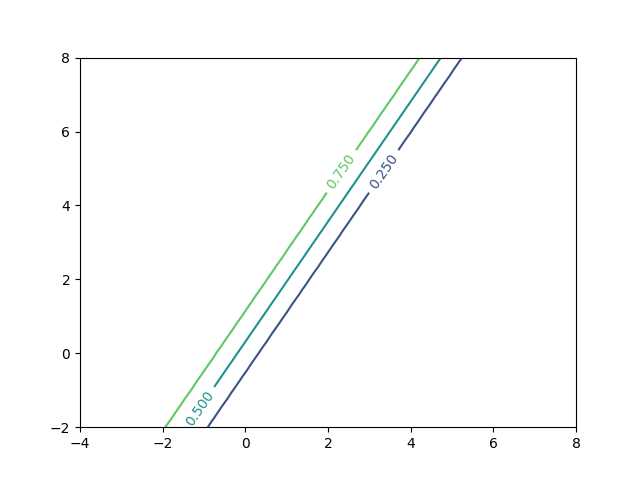
\includegraphics[scale=0.25]{y_posterior} &
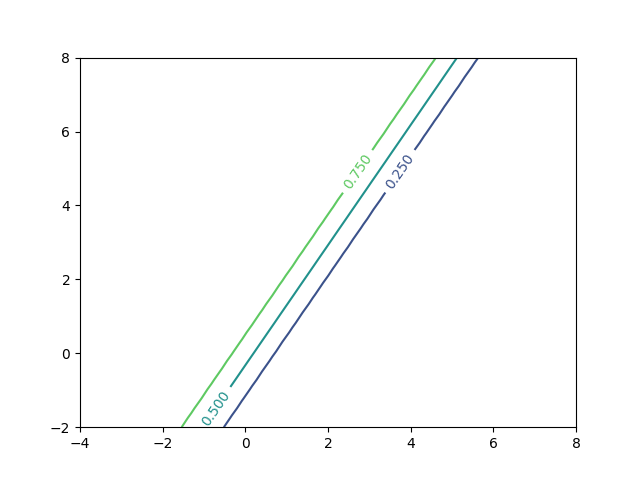
\includegraphics[scale=0.25]{z_posterior} &
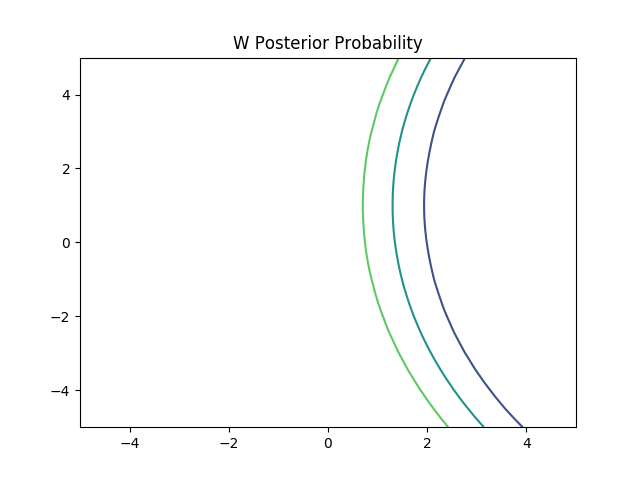
\includegraphics[scale=0.25]{w_posterior} \\
\scriptsize A & 
\scriptsize B &
\scriptsize C
\end{tabular}
\captionof{figure}{}
\end{center}

\section{Fisher LDA and ROC Curve}
Ditributions of original data, Fisher Linear Discriminant direction, and histograms of projected data are shown in Figure 3. The ROC curve and classification accuracy of Fisher LDA on several threshold values are illustrated in Figure 4.
\begin{center}
\begin{tabular}{ccc}
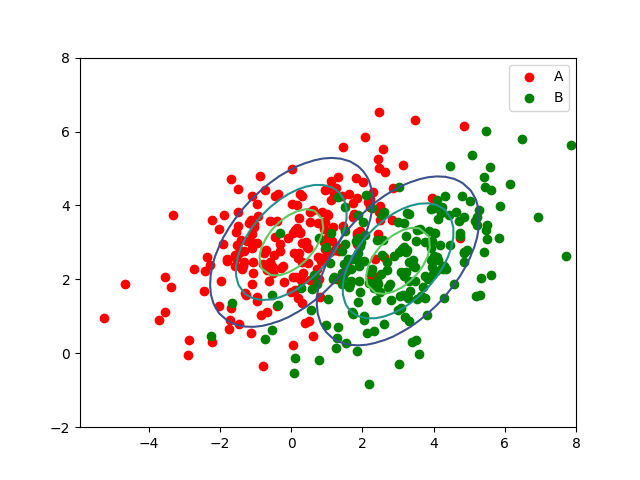
\includegraphics[scale=0.25]{flda_roc_scatter} &
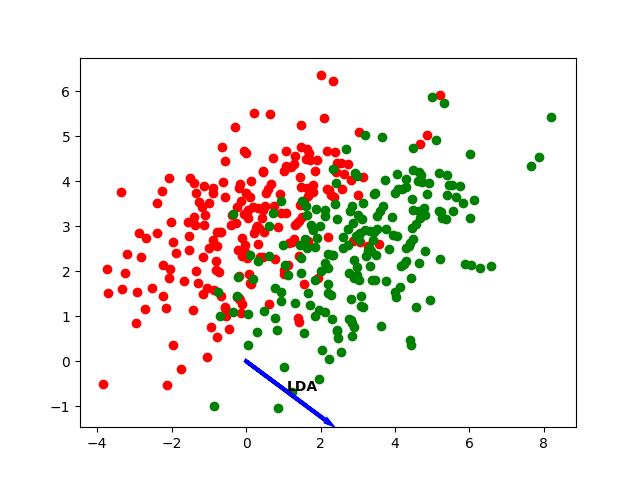
\includegraphics[scale=0.25]{discriminants} &
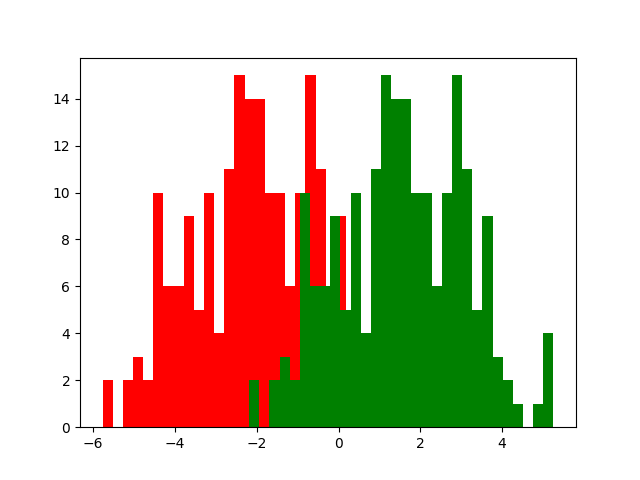
\includegraphics[scale=0.25]{flda_roc_prj_hist} \\
\scriptsize Data distribution & 
\scriptsize Fisher LDA direction &
\scriptsize Projected data distribution
\end{tabular}
\captionof{figure}{}
\end{center}

\begin{center}
\begin{tabular}{cc}
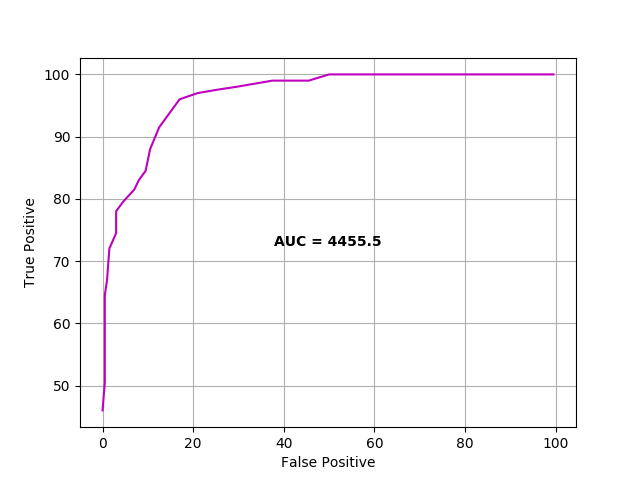
\includegraphics[scale=0.25]{roc} &
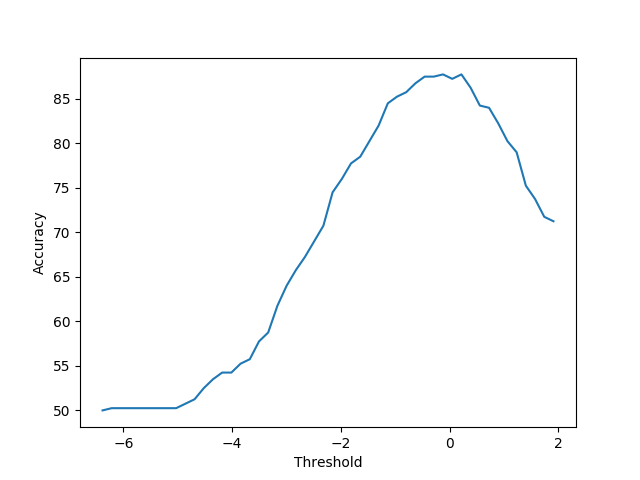
\includegraphics[scale=0.25]{accuracy}
\end{tabular}
\captionof{figure}{}
\end{center}

Figure 5. shows ROC curves of another two classifiers which project the original data onto the random direction and the direction connecting means respectively.

\begin{center}
\begin{tabular}{cc}
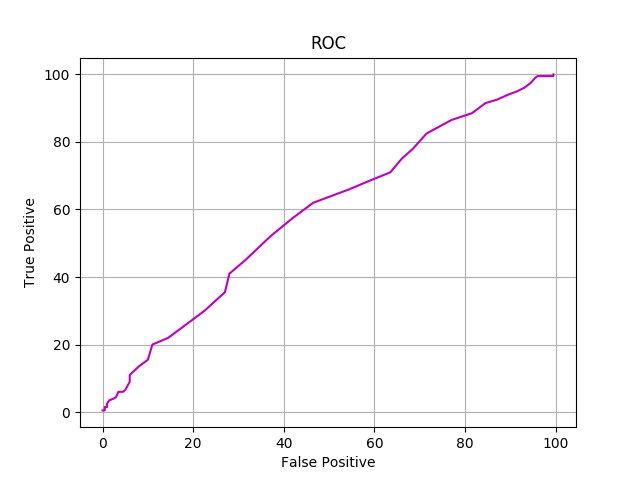
\includegraphics[scale=0.25]{roc_random_dir} &
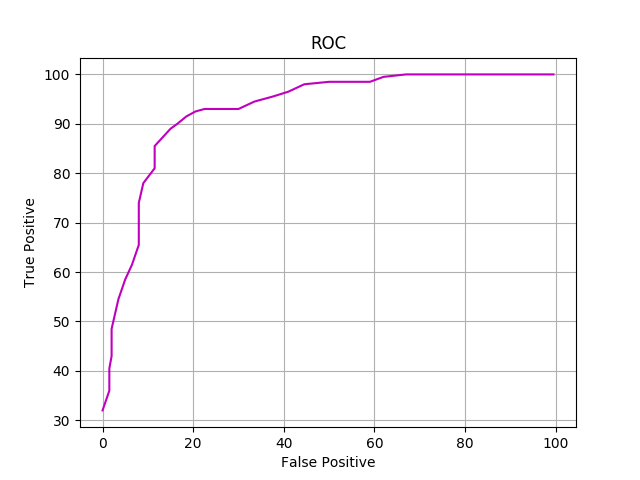
\includegraphics[scale=0.25]{roc_mean} \\
\scriptsize Random Direction &
\scriptsize Direction Connecting \textit{${m_1}$} and \textit{${m_2}$}
\end{tabular}
\captionof{figure}{}
\end{center}

\indent The area under the curve(AUC) of ROC is computed by adding True Positive of different thresholds. In other word, this area is the sum of positive samples which are correctly classified using several thresholds. This number reflects the accuracy of the classifier on the positive class. The classifier with high AUC is more likely to label a positive data point as positive than negative.  

\indent AUC of ROC curve is normally used to compare the performance of a classifiers. A model with high AUC tends to do a better job than a model which has low AUC.

\section{Mahalanobis Distance}

\begin{center}
\begin{tabular}{cc}
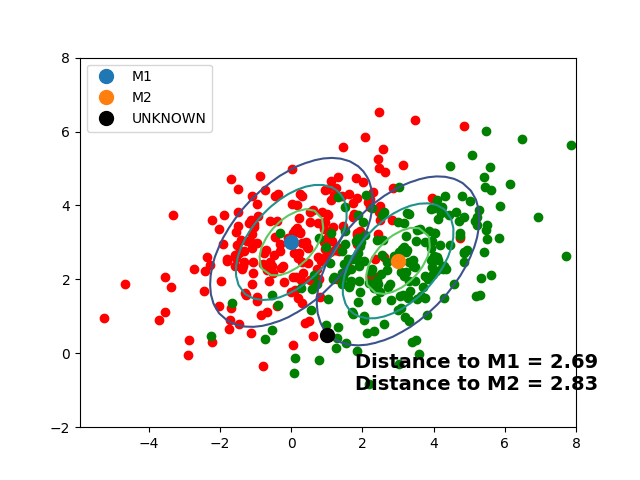
\includegraphics[scale=0.25]{distance} &
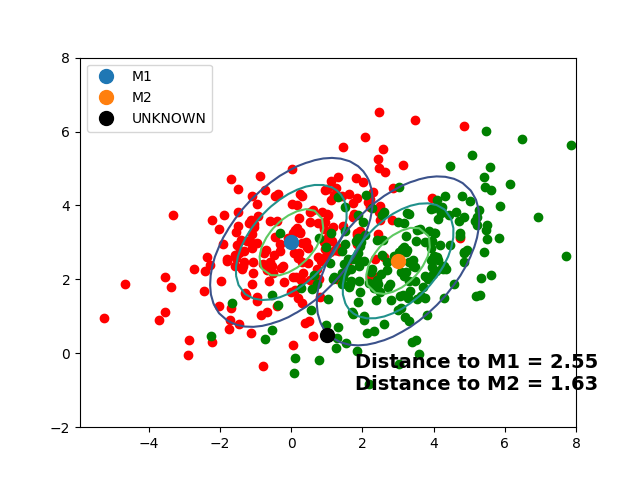
\includegraphics[scale=0.25]{m_distance} \\
\scriptsize Euclidean Distance &
\scriptsize Mahalanobis Distance \\
\end{tabular}
\captionof{figure}{}
\end{center}

The Euclidean distance-to-mean classifier will classify the unknown sample in Figure 6. as \textit{$C_1$} while the Mahalanobis distance-to-mean classifier will classify it as \textit{$C_2$}. Based on the decision boundary which is shown in Figure 1., the Mahalanobis distance-to-mean classifies is correct in this case.

\indent From the picture, although the unknown data point is geometricly closer to \textit{$m_1$} than \textit{$m_2$}, it can be observed that the point lies on the outmost contour of \textit{$C_2$} which means it is 2 standard deviation away from \textit{$m_2$}. On the other hand, the data point is located outside the outmost contour of \textit{$C_1$} so the distance to \textit{$m_1$} is more than 2 standard deviation. This observation suggests that the unknown data point is more likely to be \textit{$C_2$} than \textit{$C_1$} because both classes have a Gaussian ditribution.

\indent The above conclusion explains the difference between two classifiers. While the Euclidean distance only tells geometric distance between two data points, the Mahalanobis distance reflects the distance between a data point and the distribution as it takes covariance matrix into account.

\end{document}